\begin{frame}[t,fragile]{合成関数の微分}
  \begin{itemize}
    %\setlength{\itemsep}{1em}
  \item $f(x_1,x_2,x_3)$の$x_2$に関する偏導関数の計算
  \item 連鎖律(chain rule)
    \[
      \frac{\partial f}{\partial x_2} = \frac{\partial f}{\partial v_4} \frac{\partial v_4}{\partial x_2} + \frac{\partial f}{\partial v_5} \frac{\partial v_5}{\partial x_2} = \frac{\partial f}{\partial v_4} \frac{\partial v_4}{\partial v_2} \frac{\partial v_2}{\partial x_2} + \frac{\partial f}{\partial v_4} \frac{\partial v_4}{\partial v_3} \frac{\partial v_3}{\partial x_1} + \cdots
    \]
    \begin{itemize}
    \item $\displaystyle \frac{\partial f}{\partial x_2}$ は計算経路(全部で7つ)の和で書ける
    \end{itemize}
  \item 経路の例
    \begin{itemize}
    \item $\displaystyle \frac{\partial f}{\partial v_4} \frac{\partial v_4}{\partial v_2} \frac{\partial v_2}{\partial v_1} \frac{\partial v_1}{\partial x_2} \frac{\partial x_2}{\partial x_2} $
    \item $\displaystyle \frac{\partial f}{\partial v_5} \frac{\partial v_5}{\partial v_3} \frac{\partial v_3}{\partial x_3} \frac{\partial x_3}{\partial x_2} (=0)$
    \end{itemize}
    \vspace*{-7em} \hfill \resizebox{.3\textwidth}{!}{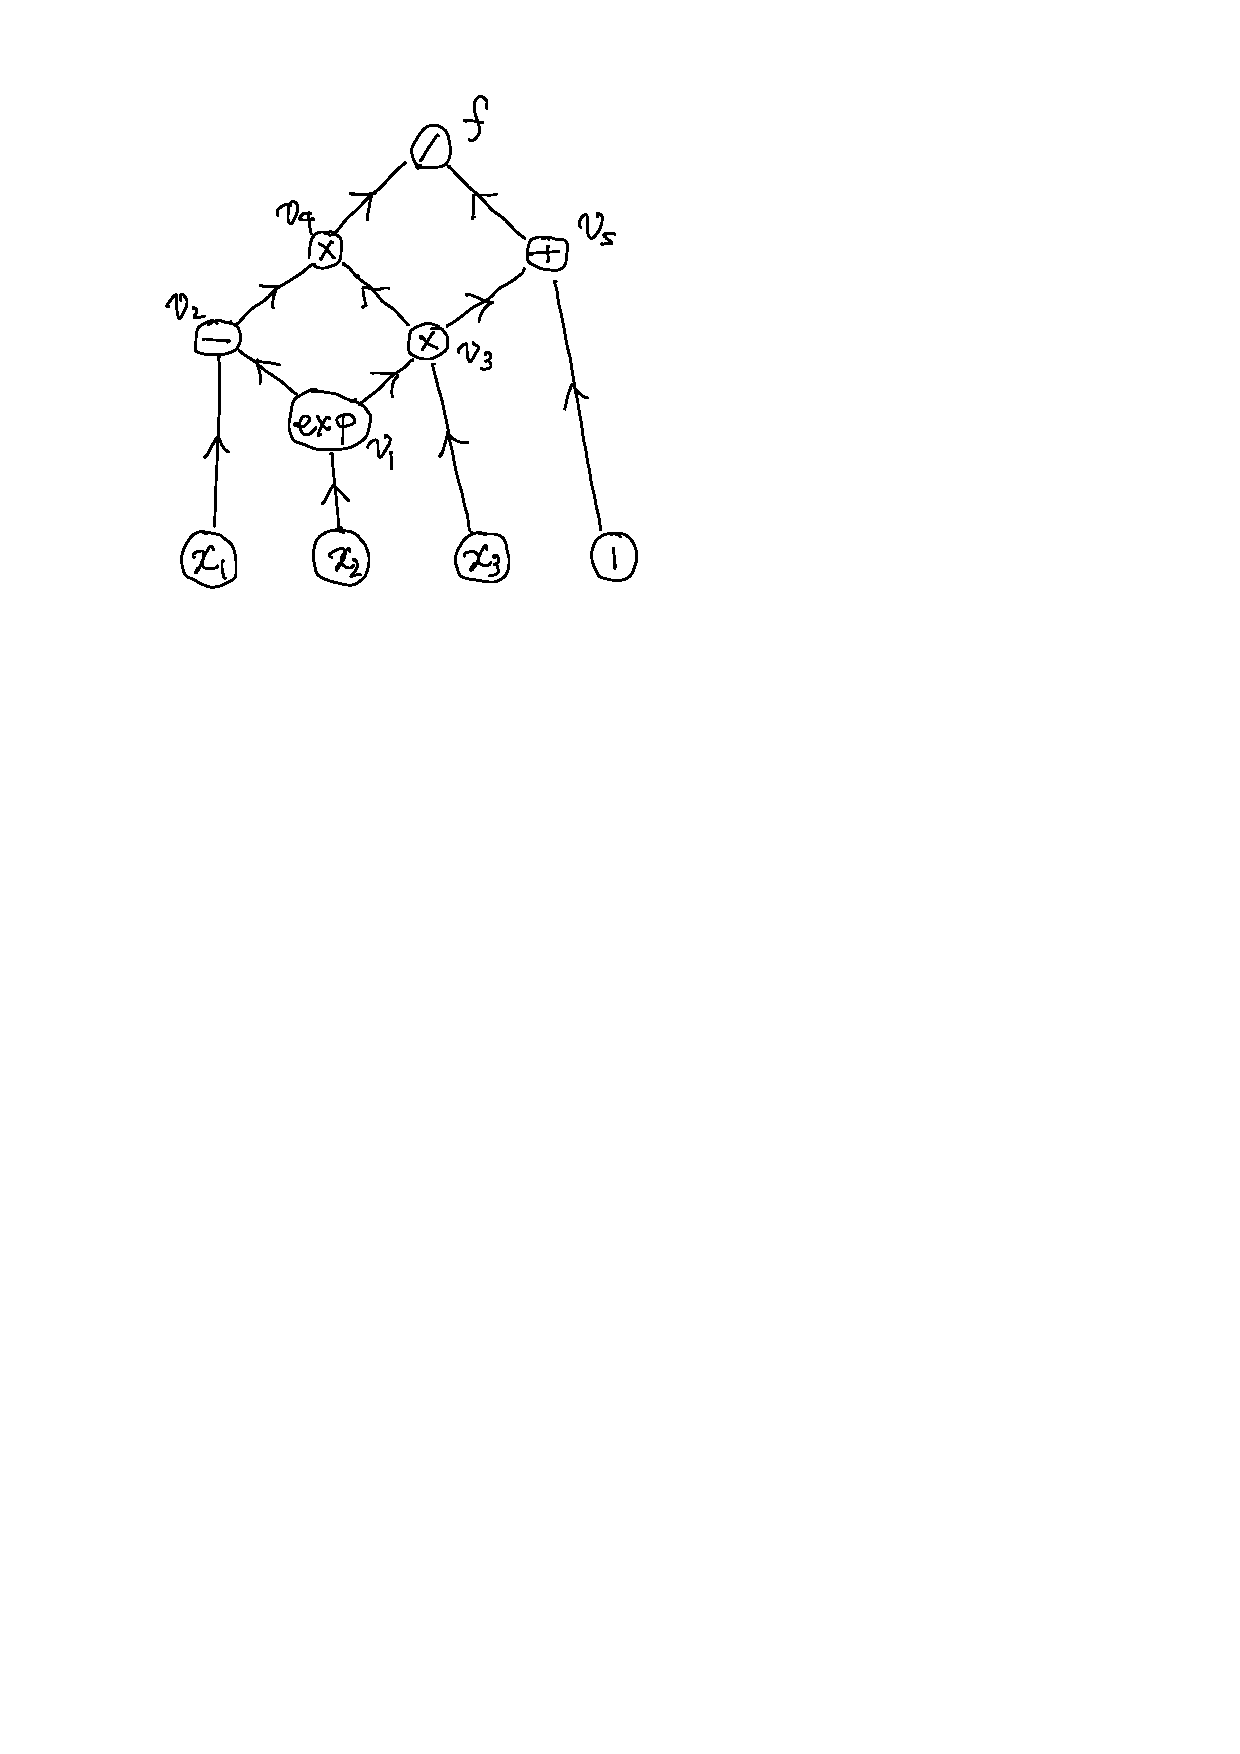
\includegraphics{image/compgraph.pdf}}
  \end{itemize}
\end{frame}
